\documentclass[a4paper, 12pt]{article}
\usepackage[utf8x]{inputenc}
\usepackage{cmap}
\usepackage[english, russian]{babel}
\usepackage{indentfirst}
\usepackage[left=20mm, top=20mm, right=20mm, bottom=20mm]{geometry}
\usepackage{tikz}
\usepackage{float}
\usepackage{amsmath, amsfonts, amssymb}
\usepackage{graphicx}
\usepackage{fancybox, fancyhdr}
\usepackage{hyperref}
\usepackage{listings}
\usepackage{caption}
\usepackage{subcaption}
\usepackage{xcolor}
\pagestyle{fancy}
\fancyhf{}
\fancyhead[L]{Лабораторная работа №3}
\fancyhead[R]{Программирование промышленных контроллеров}
\fancyfoot[C]{\thepage}
\graphicspath{{images/}}
\usetikzlibrary{patterns}
\definecolor{LightGray}{gray}{0.95}
\lstdefinestyle{pycode}{
    language=Python,
    basicstyle=\footnotesize\ttfamily,
    numbers=left,
    numberstyle=\tiny\color{gray},
    stepnumber=1,
    numbersep=5pt,
    backgroundcolor=\color{LightGray},
    showspaces=false,
    showstringspaces=false,
    showtabs=false,
    tabsize=4,
    captionpos=b,
    breaklines=true,
    breakatwhitespace=false,
    frame=none,
    rulecolor=\color{black},
    linewidth=\linewidth,
    keywordstyle=\color{red}\bfseries,
    commentstyle=\color{green!40!black},
    stringstyle=\color{blue},
    escapeinside={\%*}{*)},
    xleftmargin=0pt,
    framexleftmargin=0pt,
    framexrightmargin=0pt
}
\lstset{style=pycode}
\hypersetup{
    colorlinks=true,
    linkcolor=blue,
    filecolor=magenta,
    urlcolor=cyan,
    pdftitle={contents setup},
    pdfpagemode=FullScreen,
}
\setlength{\parskip}{1.5mm}
\setlength{\headheight}{15pt}
\setlength{\footskip}{15pt}
\allowdisplaybreaks
\DeclareMathOperator{\sinc}{sinc}
\newcommand{\frc}[2]{\raisebox{2pt}{$#1$}\big/\raisebox{-3pt}{$#2$}}

\begin{document}
    \begin{titlepage}

        \begin{center}
        
\includegraphics[width=0.3\textwidth]{itmo.png} % requires itmo.png in /images folder
        \vfill

        Федеральное государственное автономное образовательное учреждение высшего образования
        «Национальный Исследовательский Университет ИТМО»\\

        \vfill
        {\large\bf ЛАБОРАТОРНАЯ РАБОТА №3}\\
        {\large\bf ПРЕДМЕТ «ПРОГРАММИРОВАНИЕ ПРОМЫШЛЕННЫХ КОНТРОЛЛЕРОВ»}\\
        {\large\bf ТЕМА «ПЕРЕДАЧА ДАННЫХ С ПЛК ПО ПРОТОКОЛУ MODBUS TCP И УПРАВЛЕНИЕ ЧАТОТНЫМ ПРЕОБРАЗОВАТЕЛЕМ>>}
        \vfill

        \begin{flushright}
            \begin{minipage}{.45\textwidth}
                {
                    \hbox{Преподаватель:}
                    \hbox{Крылова А. А.}
                    \hbox{}
                    \hbox{Выполнили:}
                    \hbox{Румянцев А. А.}
                    \hbox{Дьячихин Д. Н.}
                    \hbox{Чебаненко Д. А.}
                    \hbox{}
                    \hbox{Факультет: СУиР}
                    \hbox{Потоки ПРОГ. ПРОМ.ЛК:}
                    \hbox{2.2, 2.1, 1.1}
                }
            \end{minipage}
        \end{flushright}

        \vfill

        Санкт-Петербург\\
        2024
        \end{center}
    \end{titlepage}
    
    \tableofcontents

    \newpage
    \section{Введение.}
    \subsection{Цель работы.}
    Разработать программу для ПЛК, которая передает в сеть
    данные с датчиков температуры и влажности по протоколу TCP. Разработать программу для управления скоростью и
    направлением вращения асинхронного двигателя с помощью частотного преобразователя.

    
    \subsection{Задания по работе.}
    \begin{enumerate}
        \item Изучить теоретическую часть работы.
        \item Реализовать модуль передачи данных в сеть на языке ST.
        \item Реализовать модуль получения, обработки и отображения данных на языке Python.
        \item Изучить документацию на частотный преобразователь.
        \item Реализовать модуль для управления частотным преобразователем по протоколу Modbus TCP.
    \end{enumerate}
    \section{Установка.}
    В данной лабораторной работе мы работали со стендом на основе ПЛК Schneider Electric Modicon M251.
    \subsection{Схема установки.}
    \begin{figure}[H]
        \centering
        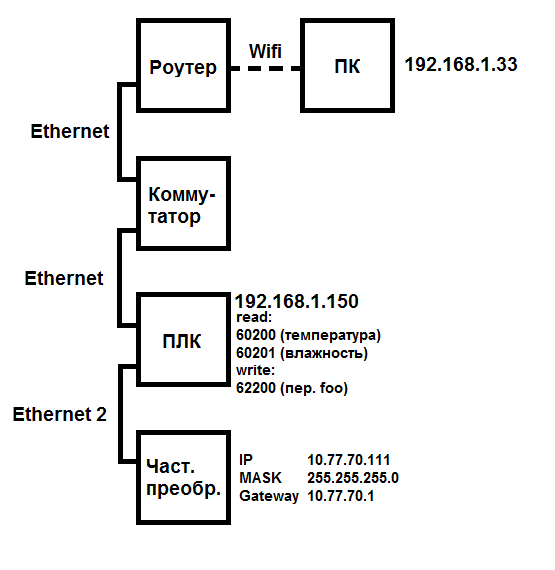
\includegraphics[scale=0.5]{scheme3.png}
        \captionsetup{skip=0pt}
        \caption{Схема протоколов стенда.}
        \label{fig:scheme}
    \end{figure}
    Так как в данной лабораторной работе мы работаем с тем же стендом, что и в предыдущей работе, то
    общая схема остается неизменной. Связь ПК и ПЛК происходит через коммутатор и Wi-Fi роутер. Во время
    выполнения работы ПК имел IP адрес 192.168.1.33 (было обнаружено с помощью команды ifconfig), а ПЛК --
    192.168.1.150. 60200 и 60201 -- адреса регистров датчика температуры и влажности соответственно, из которых можно прочитать
    данные с датчиков (для начала нужно подключиться). 62200 -- аналогично для переменной \textit{foo} (позже
    про нее будет написано подробнее), однако с той разницей, что это номер регистра для записи данных.


    \section{Теоретическая часть.}
    Modbus TCP -- открытый протокол, не зависящий от производителя используемого аппаратного обеспечения.
    Предназначен для контроля и управления оборудованием в системах несложной промышленной автоматизации.
    В частности, позволяет реализовать обмен сообщениями Modbus в локальных и глобальных вычислительных сетях
    с использованием стека протоколов TCP/IP, который часто используется для подключения к общей промышленной
    сети ПЛК, модулей ввода-вывода и <<шлюзов>>.


    Частотный преобразователь – это электронное или
    электромеханическое устройство, которое преобразует переменный ток
    (AC) одной частоты в переменный ток другой частоты. Устройство
    также может изменять напряжение, но это является второстепенным по
    отношению к его основной цели, поскольку преобразование
    напряжения переменного тока гораздо проще реализовать, нежели
    преобразование частоты.


    \section{Экспериментальная часть.}
    За основу возьмем проект лабораторной работы №2.
    
    
    \subsection{Передача данных с ПЛК по протоколу Modbus TCP.}
    В дереве проекта на вкладке \textit{Device tree} в узле
    \textit{Ethernet\_{1}} создадим объект\\\textit{ModbusTCP\_{SLAVE}\_{Device}}.
    \begin{figure}[H]
        \centering
        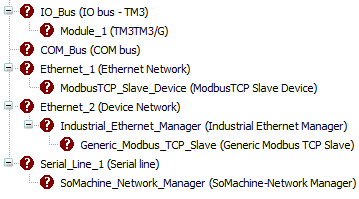
\includegraphics[scale=1.1]{modbus_tree.png}
        \captionsetup{skip=0pt}
        \caption{Созданный объект ModbusTCP\_{SLAVE}\_{Device} в дереве проекта.}
        \label{fig:mtree}
    \end{figure}


    Создадим новый список глобальных перменных в узле \textit{GVL} на
    вкладке \textit{Application tree} и добавим туда переменную \textit{foo} целого типа (остальные перменные
    будут рассмотрены позже).
    \begin{figure}[H]
        \centering
        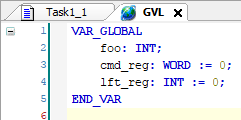
\includegraphics[scale=1.5]{global.png}
        \captionsetup{skip=0pt}
        \caption{Список глобальных переменных.}
        \label{fig:gvl}
    \end{figure}

    На вкладке \textit{Tools Tree} создадим объект \textit{Relocation Table}. В таблице \textit{Read} создадим две
    новые пустые перменные \textit{Modbus}. Нажмем на ячейку \textit{Variable} и в открывшемся диалоге найдем переменные для
    температуры и влажности из предыдущей работы. Создадим пустую переменую в таблице \textit{Write} и ассоциируем ее с
    глобальной переменной \textit{foo}, которую мы задали ранее.


    Далее напишем Python-скрипт, в котором реализуем код, необходимый для работы с ПЛК (в данном случае передача данных на ПЛК).
    \begin{lstlisting}[label=code, caption={Python-скрипт для взаимодействия с ПЛК.}]
    import time
    from pyModbusTCP import utils
    from pyModbusTCP.client import ModbusClient
        
    def read_int16(addr):
            regs = c.read_holding_registers(reg_addr=addr, reg_nb=1)
            hex_uint = utils.get_list_2comp(regs, 16)
            return hex_uint[0]
        
    c = ModbusClient(host='192.168.1.150', port=502, auto_open=True)
        
    while True:
        if c.is_open:
            temp = read_int16(60200) / 10
            hum = read_int16(60201)
            val = int(input('type int:'))
            val = min(24000, max(0, val))
            if c.write_single_register(62200, val):
                print("ok")
            print(temp, hum)
        else:
            c.open()
        time.sleep(1)
    \end{lstlisting}

    
    Данный скрипт устанавливает соединение с ПЛК по протоколу
    ModbusTCP, после чего начинает бесконечный циклический опрос
    регистров, содержащих значения температуры и влажности, а также
    запись введенных пользователем в консоль значений (\textit{val}) в регистр,
    ассоциированный с глобальной переменной проекта. При этом значение переменной
    не может превысить $24000$ или быть ниже $0$.


    После мы загрузили программу в ПЛК и запустили ее, тем самым убедившись
    в том, что все скомпилировалось без ошибок, значение глобальной переменной в узле \textit{GVL} изменяется всегда, когда пользователь
    вводит некоторое значение в консоль, данные температуры и влажности отображаются в консоли.


    Мы приравняли переменную \textit{foo} к переменной \textit{motor}, чтобы при передаче данных в первую из них вторая подбирала это значение и передавала на мотор.
    Программа корректно выполнялась -- мотор вращался с той скоростью, которую пользователь ввел в консоль на своем ПК. Подаваемые значения не превышали заданный диапазон значений и не были
    ниже его.

    
    \subsection{Управление частотным преобразователем.}
    Данное задание является продолжением предыдущего. В дерево устройств добавим устройство
    \textit{Generic\_{ModbusTCP}\_{Slave}} к узлу \textit{Ethernet\_{2}} (см. рис. \ref{fig:mtree}).
    После этого зададим IP адрес частотного преобразователя $10.77.70.110$ (см. рис. \ref{fig:scheme}).


    Далее на вкладке \textit{Modbus TCP Channel Configuration} нажмем кнопку \textit{Add Channel} и
    в открывшемся диалоговом окне зададим два канала управления для включения частотного преобразователя
    (регистр CMD, адрес 8501) и частоты (регистр LFR, адрес 8502).


    Для описанных ранее регистров в узле \textit{GVL} создадим две новые глобальные переменные -- \textit{cmd\_{reg}}
    и \textit{ifr\_{reg}} (см. рис. \ref{fig:gvl}). После этого ассоциируем их с каналами управления на вкладке
    \textit{ModbusTCPSlave I/O Mapping}.
    \begin{figure}[H]
        \centering
        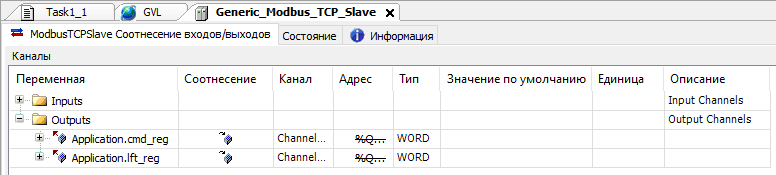
\includegraphics[scale=0.8]{gmtcps.png}
        \captionsetup{skip=0pt}
        \caption{ModbusTCPSlave I/O Mapping (Outputs).}
        \label{fig:gmtcps}
    \end{figure}


    На вкладке \textit{Application Tree} добавим новую программу с именем \textit{TASK1\_{1}}. Создадим в ней
    локальную переменную \textit{counter} и напишем программу для управления частотным преобразователем.
    \begin{figure}[H]
        \centering
        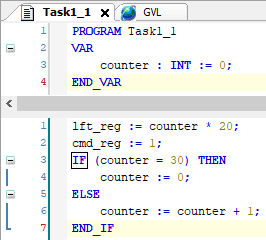
\includegraphics[scale=1.3]{code.png}
        \captionsetup{skip=0pt}
        \caption{Программа для управления частотным преобразователем.}
        \label{fig:codeplc}
    \end{figure}


    Создадим циклическую задачу в MAST и ассоциируем ее с программой управления скоростью частотного преобразователя.
    Интервал поставим в одну секунду, чтобы значения не обновлялись слишком часто.
    \begin{figure}[H]
        \centering
        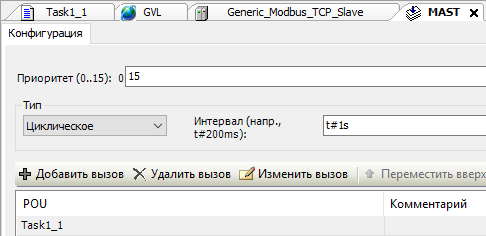
\includegraphics[scale=1.3]{cycl.png}
        \captionsetup{skip=0pt}
        \caption{Циклическая задача в MAST, к которой привязан TASK1\_{1}.}
        \label{fig:cycl}
    \end{figure}


    Программа работает следующим образом. Для включения
    частотного преобразователя необходимо в нулевой бит
    регистра CMD записать значение 1, то есть в нашем случае
    просто присвоить значение 1 всей переменной. Изначальная
    частота вращения двигателя равна 0 (переменная \textit{ifr\_{reg}}).
    На каждом цикле программы мы берем локальный счётчик,
    умножаем его значение на 20, а затем записываем в регистр
    частоты, после чего инкрементируем счётчик, а при
    достижении значения 30 обнуляем его. Таким образом частота
    плавно увеличивается от 0 до 600 Гц.
    При этом скорость вращения двигателя будет зависеть от его
    паспортных характеристик, например, если на шильдике
    двигателя написано 50 Гц, 1400 об/мин., частота будет меняться
    в диапазоне от 0 до 2800 об/мин.


    После мы запустили программу на стенде ПЛК и частотный преобразователь выполнял действия в
    соответствии с ранее описанным алгоритмом. Данные о частоте мы отслеживали с помощью специального
    пульта, прилагаемого к предоставленному нам ПЛК.


    \section{Выводы о проделанной работе.}
    В ходе лабораторной работы мы разработали программу для ПЛК на языке ST, которая передает в сеть данные с датчиков
    температуры и влажности по протоколу TCP, а также принимает значения для управления скоростью мотора. Также мы
    написали программу для получения, обработки и отображения данных на языке Python. В конце мы поработали с частотным
    преобразователем и разработали программу для управления скоростью и направлением вращения асинхронного двигателя
    с помощью частотного преобразователя по протоколу Modbus TCP.
\end{document}